%% This is file `elsarticle-template-1-num.tex',
%%
%% Copyright 2009 Elsevier Ltd
%%
%% This file is part of the 'Elsarticle Bundle'.
%% ---------------------------------------------
%%
%% It may be distributed under the conditions of the LaTeX Project Public
%% License, either version 1.2 of this license or (at your option) any
%% later version.  The latest version of this license is in
%%    http://www.latex-project.org/lppl.txt
%% and version 1.2 or later is part of all distributions of LaTeX
%% version 1999/12/01 or later.
%%
%% The list of all files belonging to the 'Elsarticle Bundle' is
%% given in the file `manifest.txt'.
%%
%% Template article for Elsevier's document class `elsarticle'
%% with numbered style bibliographic references
%%
%% $Id: elsarticle-template-1-num.tex 149 2009-10-08 05:01:15Z rishi $
%% $URL: http://lenova.river-valley.com/svn/elsbst/trunk/elsarticle-template-1-num.tex $
%%
%%\documentclass[preprint,12pt]{elsarticle}

%% Use the option review to obtain double line spacing
%% \documentclass[preprint,review,12pt]{elsarticle}

%% Use the options 1p,twocolumn; 3p; 3p,twocolumn; 5p; or 5p,twocolumn
%% for a journal layout:
%% \documentclass[final,1p,times]{elsarticle}
%% \documentclass[final,1p,times,twocolumn]{elsarticle}
%% \documentclass[final,3p,times]{elsarticle}

 \documentclass[final,3p,times,twocolumn]{elsarticle}
% \documentclass[review,3p,times,twocolumn,sort&compress]{elsarticle}

%% \documentclass[final,5p,times]{elsarticle}
%% \documentclass[final,5p,times,twocolumn]{elsarticle}

%% if you use PostScript figures in your article
%% use the graphics package for simple commands
%% \usepackage{graphics}
%% or use the graphicx package for more complicated commands
%% \usepackage{graphicx}
%% or use the epsfig package if you prefer to use the old commands
%% \usepackage{epsfig}

%% The amssymb package provides various useful mathematical symbols
\usepackage{amssymb}
%% The amsthm package provides extended theorem environments
%% \usepackage{amsthm}

%% The lineno packages adds line numbers. Start line numbering with
%% \begin{linenumbers}, end it with \end{linenumbers}. Or switch it on
%% for the whole article with \linenumbers after \end{frontmatter}.
\usepackage{lineno}


%% natbib.sty is loaded by default. However, natbib options can be
%% provided with \biboptions{...} command. Following options are
%% valid:

%%   round  -  round parentheses are used (default)
%%   square -  square brackets are used   [option]
%%   curly  -  curly braces are used      {option}
%%   angle  -  angle brackets are used    <option>
%%   semicolon  -  multiple citations separated by semi-colon
%%   colon  - same as semicolon, an earlier confusion
%%   comma  -  separated by comma
%%   numbers-  selects numerical citations
%%   super  -  numerical citations as superscripts
%%   sort   -  sorts multiple citations according to order in ref. list
%%   sort&compress   -  like sort, but also compresses numerical citations
%%   compress - compresses without sorting
%%
%% \biboptions{comma,round}

% \biboptions{}

% HPS stuff
%\usepackage{url}
\usepackage{hyperref}
%\usepackage{fancyhdr}
\usepackage{color}
%\usepackage{multicol}
\newcommand{\Aprimebold}{\ensuremath{\mathrm{\mathbf{A}}^\prime}}
\newcommand{\Aprime}{\ensuremath{\mathrm{A}^\prime}}
%\newcommand{\Aprime}{A\ensuremath{^\prime}}
\newcommand{\ee}{e$^+$e$^-$}
\newcommand{\fluenceunit}{1~MeV~neutron~equivalent/cm\ensuremath{^2}}
\newcommand{\geant}{{\sc Geant4}}
\newcommand{\egs}{{\sc EGS5}}
\newcommand{\moliere}{Moli\`{e}re}
%\include{affiliations}

\journal{Nuclear Instruments and Methods in Physics Research Section A}

\begin{document}

\begin{frontmatter}


%% Title, authors and addresses

%% use the tnoteref command within \title for footnotes;
%% use the tnotetext command for the associated footnote;
%% use the fnref command within \author or \address for footnotes;
%% use the fntext command for the associated footnote;
%% use the corref command within \author for corresponding author footnotes;
%% use the cortext command for the associated footnote;
%% use the ead command for the email address,
%% and the form \ead[url] for the home page:
%%
%% \title{Title\tnoteref{label1}}
%% \tnotetext[label1]{}
%% \author{Name\corref{cor1}\fnref{label2}}
%% \ead{email address}
%% \ead[url]{home page}
%% \fntext[label2]{}
%% \cortext[cor1]{}
%% \address{Address\fnref{label3}}
%% \fntext[label3]{}



\title{Rate of FPGA Single Event Upset from Neutron Exposure}
%\title{
%\begin{flushleft}
%%       \mbox{\textmd{ \normalsize -PUB-13/020 }}
 %       \mbox{\textmd{ \normalsize SLAC-PUB-15999 }}
  %     \end{flushleft}
%{
%The Heavy Photon Search Test Detector
%}
%}

%%%%%%%%%%%%%%%%%%%%%%%%%%%%%%%%%%%%%%%%%%%%%%%%%%
%% use optional labels to link authors explicitly to addresses:
%% \author[label1,label2]{<author name>}
%% \address[label1]{<address>}
%% \address[label2]{<address>}


\newcommand{\red[1]}{{\color{red}{\bf #1}}}
\newcommand{\JLAB}{Thomas Jefferson National Accelerator Facility, Newport News, Virginia 23606}
\newcommand{\UCSC}{Santa Cruz Institute for Particle Physics, University of California, Santa Cruz, CA 95064}
\newcommand{\SLAC}{SLAC National Accelerator Laboratory, Menlo Park, CA 94025}



\author[JLAB]{S. Boyarinov} 
\author[SLAC]{ G. Haller} 
\author[SLAC]{P. Hansson Adrian\corref{corrauthor}}
\ead{phansson@slac.stanford.edu}
\author[SLAC]{ R. Herbst} 
\author[SLAC]{ J. Jaros} 
\author[UCSC]{ O. Moreno}
\author[SLAC]{ T. Nelson} 
\author[SLAC]{ B. Reese} 
\author[SLAC]{ S. Uemura} 
%
%
%
%
%
%
 %
%
%
%
%
%
%
%
%

\address[JLAB]{\JLAB}
\address[UCSC]{\UCSC}
\address[SLAC]{\SLAC}                                 


\cortext[corrauthor]{Corresponding author.}




%\author[slac]{Per Hansson Adrian\corref{cor1}}
%\ead{phansson@slac.stanford.edu}
%\address[slac]{SLAC National Accelerator Laboratory, 94025, Menlo Park, CA, USA}

%%%%%%%%%%%%%%%%%%%%%%%%%%%%%%%%%%%%%%%%%%%%%%%%%%


\begin{abstract}
Rates of single event upset (SEU) events in FPGAs in a rich neutron background environment are reported based on data from the 
Heavy Photon Search (HPS) experiment running at Thomas Jefferson National Accelerator Facility (JLab). The HPS experiment deploys 
ten Xilinx Artix-7 FPGAs distributed between 10 and 70~cm from a thin fixed-target foil and approximately 15~cm from the CEBAF electron beam 
in Hall~B. The resulting neutron doses during steady state running of the HPS experiment are of the order of X~neutrons$/cm^{2}$/s. Neutron 
doses are based on simulations using FLUKA and validated with neutron detectors. In total X number of SEUs was recorded during steady state 
running and the estimate During the 2016 spring run a total of Y SEUs were detected over an active detection time of approximately X~days which 
corresponds to X Failure In Time per Mb. This paper describes the estimation of the radiation environment and the error detection mechanism and 
compares them to existing data from other applications. 
\end{abstract}

\begin{keyword}
%% keywords here, in the form: keyword \sep keyword
FPGA \sep Xilinx \sep Artix-7 \sep single event upset \sep soft error \sep SEU
%% MSC codes here, in the form: \MSC code \sep code
%% or \MSC[2008] code \sep code (2000 is the default)

\end{keyword}


\end{frontmatter}

 %\linenumbers
 
\tableofcontents
%\clearpage
%\newpage
\newpage

%%
%% Start line numbering here if you want
%%
%\linenumbers

%% main text

\section{Introduction}
% The very first letter is a 2 line initial drop letter followed
% by the rest of the first word in caps.
% 
% form to use if the first word consists of a single letter:
% \IEEEPARstart{A}{demo} file is ....
% 
% form to use if you need the single drop letter followed by
% normal text (unknown if ever used by IEEE):
% \IEEEPARstart{A}{}demo file is ....
% 
% Some journals put the first two words in caps:
% \IEEEPARstart{T}{his demo} file is ....
% 
% Here we have the typical use of a "T" for an initial drop letter
% and "HIS" in caps to complete the first word.

%%%%%%%%%%%%%%%%%%%%%%%%%%%%%%%%%%%%%%%%%%%%%%%%%%%%%%%%%%%%%%%%%%%%%%%%

Reliability of electronic devices placed in environments with large radiation is of continuous importance 
to a wide variety of applications in industries such as aerospace and defense and satellite- or accelerator 
based  basic science experiments. With program lifetimes that span over decades and hard requirements on 
reliability the technology choices are complex and evaluated based on a variety of criteria. For accelerator-based 
experiments stringent requirements on data corruption rates requires experiments to estimate and evaluate 
different technologies available for deployment in such environments. Reconfigurable FPGAs are now a cornerstone of 
the data processing for most accelerator-based experiment with mature products where vendors provide long life-cycle 
support as well as radiation-tolerant designs. The FPGAs offer advantages of low power, high reliability and almost  
unlimited number of circuit programming lowering the engineering risks and increasing flexibility compared to custom ASICs. 
In practice, modern experiments often deploy both custom ASICs and FPGAs as described in this paper.

The effect of radiation in electronics is a rich subject handled in depth in Ref.~{x-y} and depends on a wide variety of parameters that includes the 
exact technology and of course what type of radiation that is being considered. This paper has two main goals: one is the describe the 
estimation of neutron induced errors in Xilinx FPGAs detected from a real-world particle physics experiment and the other is to provide 
a comparison data point for other, similar, experiment to normalize their expected rates of errors of this kind. For the latter, we compare 
our estimation with information available from tests under supervision of Xilinx. 

The data we present in this paper comes from the Heavy Photon Search experiment (HPS) which is a fixed-target 
experiment~\cite{proposal_full} at the the CEBAF accelerator at the Thomas Jefferson National Accelerator Facility (JLab). The HPS 
experiment deploys Xilinx FPGAs close the high intensity electron beam target and beamline leading to large neutron fluxes. Using the 
Xilinx soft error detection mechanism we were able to measure SEUs and compute failure probabilities using data-verified neutron 
flux simulations. 

This paper is organized as follows. Section~\ref{sec:hps} gives a brief introduction of the HPS experiment and the location and usage of the 
the FPGAs. Secion~\ref{sec:flux} explains the modeling of the radiation environment and the estimates of the neutron 
flux used to compute the failure rate probability.  The error detection mechanism is described in Sec.~\ref{sec:sem} and the measured 
SEUs are detailed turned into a failure rate probability from the results in Sec.~\ref{sec:results}. 


\section{The HPS Experiment and its FPGAs}
\label{sec:hps}
The HPS experiment deploys ten Xilinx Artix-7 FPGAs (actually Art. nr here) to process data from a total of 23,004 channels spread out on 
36 silicon microstrip sensors readout by a analog front end ASICs. The FPGAs are 
also used to configure the ASICs and to monitor and control power. 
The experiment, in Hall~b at JLab, places the sensors only 10~cm behind the thin, 0.25\% radiation lengths, Tungsten target foil with the core of the 
scattered beam as close as 0.5~mm from the sensor edges.  The target is illuminated by the CEBAF nearly continuous electron beam with 
currents ranging from 50-300~nA. The proximity to the beam and practical considerations has the sensors placed inside an existing magnet 
with a vacuum chamber part of the accelerator beam vacuum. To minimize cable lengths and avoid excessive vacuum penetration counts the 
first stage data processing after the analog front end ASIC are ten so-called Front End Boards (FEBs). These share the load of digitizing and 
packaging data from the 36 sensors before sending it out on high-speed optical links to the DAQ platform 30~m away. The FEBs also have to 
configure the ASICs in addition to control power and monitor the state of the sensor electronics inside the vacuum chamber. The only realistic 
choice for the FEBs was to use an FPGA to handle the wide set of tasks. 

Continue here...the below are placeholders with too much information. Not sure we need any of this except for a description of how resources 
are used in the FGPA?

\subsection{Front End Board}
\label{sec:feb}
The FEB serves two purposes: distribute power to the hybrids and digitize analog readout data from each hybrid APV25. Its design and placement 
inside the SVT vacuum chamber is motivated by a desire to reduce vacuum penetration count and analog signal length. The design centers around a 
Xilinx Artix-7 FPGA to interface to the ADCs, transmit digitized data up-stream, distribute clock, trigger, and I$^2$C communication to the hybrids, and 
control and monitor hybrid power distribution.
Deployment of FEBs inside the SVT chamber presents a number of challenges. Due to the presence of a 2~T magnetic field, great care was taken with 
the design of all onboard power regulators. Ferrite core inductors commonly used with DC-DC switching regulators will saturate in such high fields and 
lose effectiveness. It was also desired that no magnetically conduct-ing material be used on the board, so as not to distort the magnetic field inside the 
chamber. This necessitated the use air-core inductors in power regulation circuits and throughout the board.
Radiation is also a concern inside of the SVT chamber. Beam interactions with the Tungsten target produce both neutrons and x-rays, which can 
have adverse effects on the FEBs. Neutrons can cause Single Event Upsets (SEUs) in the digital circuits of the FPGA, and x-ray doses can degrade 
integrated circuits over time. Simulations indicated that these sources should be within acceptable limits, but additional measures were taken just in 
case. A Borated-Polyethylene shield was installed around the FEBs to block neutrons, and the boards are installed on a serviceable custom cooling 
plate so that they can be replaced if needed.
\begin{figure}[]
\centering
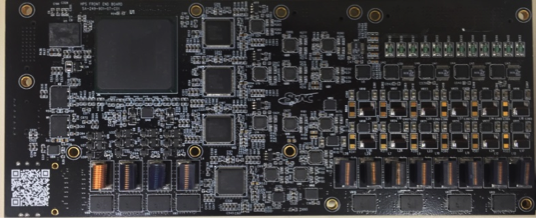
\includegraphics[width=3.0in]{feb.png}
\caption{One COB ATCA blade used in the RCE platform.}
\label{fig:cob}
\end{figure}
Each FEB connects to 4 hybrids, for a total of 20 APV25 analog channels. A preamplifier circuit converts the �4 mA signal from each APV25 into a 
voltage scaled to the range of the AD9252 14-bit ADC. The ADC sample clock runs at the same frequency as the APV25 clock, but has a 
programmable phase offset so that each sample can be taken at the center-point be-tween analog transitions.
The FPGA monitors each APV25 ADC stream looking for readout frames. Every readout frame is then sent upstream by a multi-gigabit transceiver 
(MGT). The FEB has four upstream-only MGTs, with one dedicated to each hybrid. By dropping the two least significant noise bits from each ADC 
sample, each hybrid�s readout data can be packed on to a 3.125 Gbps link at rates approaching 50~kHz. Performing APV25 frame recovery on the 
FPGA in this manner allows the link speed to scale with the trigger rate, as well as robust error recovery on the upstream end. At the maximum trigger 
rate of 48.7~kHz, the combined data output rate from all of the FEBs is 89.6 Gbps.
An additional full duplex MGT provides for configuration, trigger, and clock to be received from the upstream system. This link operates in a special 
fixed-latency mode so that every FEB in the system can recover the same 125~MHz beam-synchronous clock with minimal skew. The recovered clock is 
divided on each FEB to create the 41.667~MHz APV25 and ADC clocks. Triggers and clock alignment commands can be sent down these links with a 
guaranteed latency, assuring that all APV25s in the system receive the same clock and triggers in lockstep with each other.
The FEB is also responsible for distributing and monitoring hybrid power. Switched-mode regulators are used to efficiently step down a 6V reference to 
three intermediate voltages � 2.9V, 2.9V and 1.4V. Linear regulators then convert these voltages into the 2.5V (DVDD), 2.5V (AVDD) and 1.25V 
needed by each hybrid. AD5144 SPI digital potentiometers placed in the resistor feedback of each regulator allow for all of the regulated voltages to be 
trimmed by the FPGA to account for cable drops. LTC2991 I$^2$C ADCs are deployed to monitor the output voltage, feedback voltage and output 
current on each of the twelve hybrid voltage outputs. All of these monitors are accessible on the control link, and are sampled every second for delivery 
to EPICS slow controls.
\begin{figure}[]
\centering
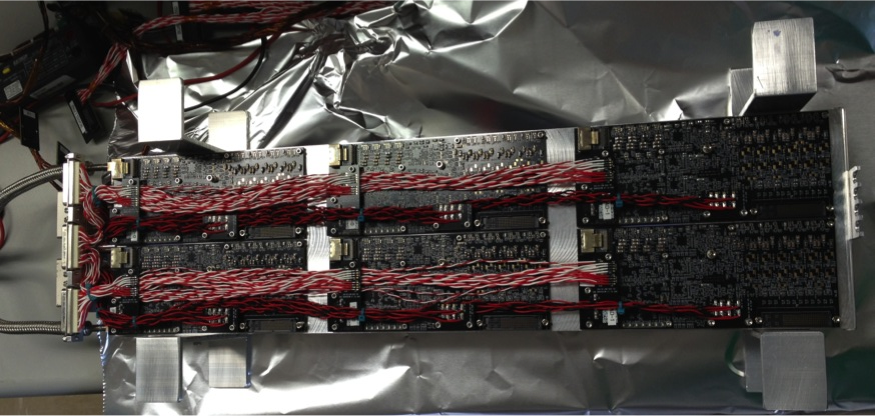
\includegraphics[width=3.0in]{febs.png}
\caption{The partially cabled data acquisition front end boards  screwed to the aluminum support plate before installation .}
\label{fig:febs}
\end{figure}




\section{Radiation Environment}
\label{sec:flux}

\subsection{Overview}

\subsection{Simulation}

\subsection{Normalization using Neutron Detectors}

\section{Single Event Upset Detection and Monitoring}
\label{sec:sem}
Description of how, what and when we detect. 


\section{Results}
\label{sec:results}

Normalization of the neutron. 

The probability of a SEU, $p$, in HPS is given by,
\begin{equation}
p = \frac{N}{\Phi}\times Q_{tot}
\end{equation}
where $N$ is the observed number of SEUs, $\Phi$ is the neutron flux per cm$^{2}$ per Coulomb of charge at the FPGAs and $Q_{tot}$ is the 
total integrated charge while the error detector was enabled during stable running. 
\begin{itemize}
\item 
Pelle finds $N$ and $Q_{tot}$. 
\item
Takashi finds $\Phi$
\item
Ben finds out how the error probabilities are defined in industry e.g. FIT/Mb and the like and then we'll figure out how we compute it. 
\end{itemize}



%\begin{figure}[]
%\centering
%\includegraphics[width=3.5in]{svt-layout.png}
%\caption{A rendered overview of the SVT installed on the beamline.}
%\label{fig:layout}
%\end{figure}
%\begin{table}
%\centering
%\begin{tabular}{|lcc|}
%\hline
%Layer $\rightarrow$& 1-3 & 4-6 \\ 
%\hline
%$z$ pos. (cm)  & 10-30 & 50-90  \\
%\hline
%\end{tabular}
%\caption{Main tracker parameters.}
%\label{tab:layout}
%\end{table}




\section{Conclusion}





\section{Acknowledgements}
Thanks you.


%% The Appendices part is started with the command \appendix;
%% appendix sections are then done as normal sections
%% \appendix

%% \section{}
%% \label{}

%% References
%%
%% Following citation commands can be used in the body text:
%% Usage of \cite is as follows:
%%   \cite{key}          ==>>  [#]
%%   \cite[chap. 2]{key} ==>>  [#, chap. 2]
%%   \citet{key}         ==>>  Author [#]

%% References with bibTeX database:

\bibliographystyle{model1-num-names}
%\bibliography{<your-bib-database>}
\bibliography{hps-svt-seu-paper}

%% Authors are advised to submit their bibtex database files. They are
%% requested to list a bibtex style file in the manuscript if they do
%% not want to use model1-num-names.bst.

%% References without bibTeX database:

% \begin{thebibliography}{00}

%% \bibitem must have the following form:
%%   \bibitem{key}...
%%

% \bibitem{}

% \end{thebibliography}


\end{document}

%%
%% End of file `elsarticle-template-1-num.tex'.
